\documentclass[a4paper,14pt]{extarticle} 
\usepackage[a4paper,top=1.5cm, bottom=1.5cm, left=2cm, right=1cm]{geometry}
%\usepackage[T2A]{fontenc}
%\usepackage[english, russian]{babel}
\usepackage{graphicx}
\graphicspath{{./pics/}}
\DeclareGraphicsExtensions{.pdf,.png,}

\usepackage{fontspec}
\setmainfont{Times New Roman}
\setsansfont{FreeSans}
\setmonofont{FreeMono}
\renewcommand{\baselinestretch}{1.5}
\usepackage{polyglossia}
\setdefaultlanguage{russian}
\setotherlanguages{english,russian}
\usepackage{setspace}
\usepackage[many]{tcolorbox}

\begin{document}
    \begin{center}
        \thispagestyle{empty}
        \begin{singlespace}
        ФЕДЕРАЛЬНОЕ АГЕНТСТВО СВЯЗИ

        ФЕДЕРАЛЬНОЕ ГОСУДАРСТВЕННОЕ БЮДЖЕТНОЕ ОБРАЗОВАТЕЛЬНОЕ

        УЧРЕЖДЕНИЕ ВЫСШЕГО ОБРАЗОВАНИЯ

        «САНКТ-ПЕТЕРБУРГСКИЙ ГОСУДАРСТВЕННЫЙ УНИВЕРСИТЕТ ТЕЛЕКОММУНИКАЦИЙ ИМ. ПРОФ. М.А. БОНЧ-БРУЕВИЧА»

        (СПбГУТ)
        \end{singlespace}
        \vspace{-1ex}
        \rule{\textwidth}{0.4pt}
        \vspace{-5ex}

        Факультет \underline{Инфокоммуникационных сетей и систем}

        Кафедра \underline{Защищенных систем связи}
        \vspace{10ex}

        \textbf{Лабораторная работа №7}\\
        МОНИТОРИНГ СОБЫТИЙ И ПРОИЗВОДИТЕЛЬНОСТЬ СИСТЕМЫ 


    \end{center}
    \vspace{4ex}
    \begin{flushright}
    \parbox{10 cm}{
    \begin{flushleft}
        Выполнили студенты группы ИКТЗ-83:

        \underline{Громов А.А., Миколаени М.С.} \hfill \rule[-0.85ex]{0.1\textwidth}{0.6pt}\\
        \vspace{-1ex}
        \footnotesize \textit{ (Ф.И.О., № группы) \hfill (подпись)} \normalsize

        Проверил:

        \underline{Цветков А.Ю.} \hfill \rule[-0.85ex]{0.1\textwidth}{0.6pt}\\
        \vspace{-1ex}
        (\footnotesize \textit{уч. степень, уч. звание, Ф.И.О.) \hfill (подпись)} \normalsize

    \end{flushleft}
    }
    \end{flushright}
    \begin{center}
        \vfill
        Санкт-Петербург

        2020

    \end{center}
    \newpage

    \textbf{Цель лабораторной работы:}
    \vspace{-2em}
    \begin{enumerate}
        \begin{singlespace}
            \item Изучить оснастку "Просмотр событий"
            \item Ознакомиться с "Диспетчер задач" 
        \end{singlespace}
    \end{enumerate}

    Схема сети:
    \begin{center}
        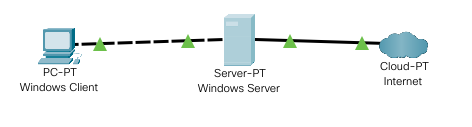
\includegraphics{net.png}
    \end{center}

    \textbf{пункт 6}
    \begin{center}
        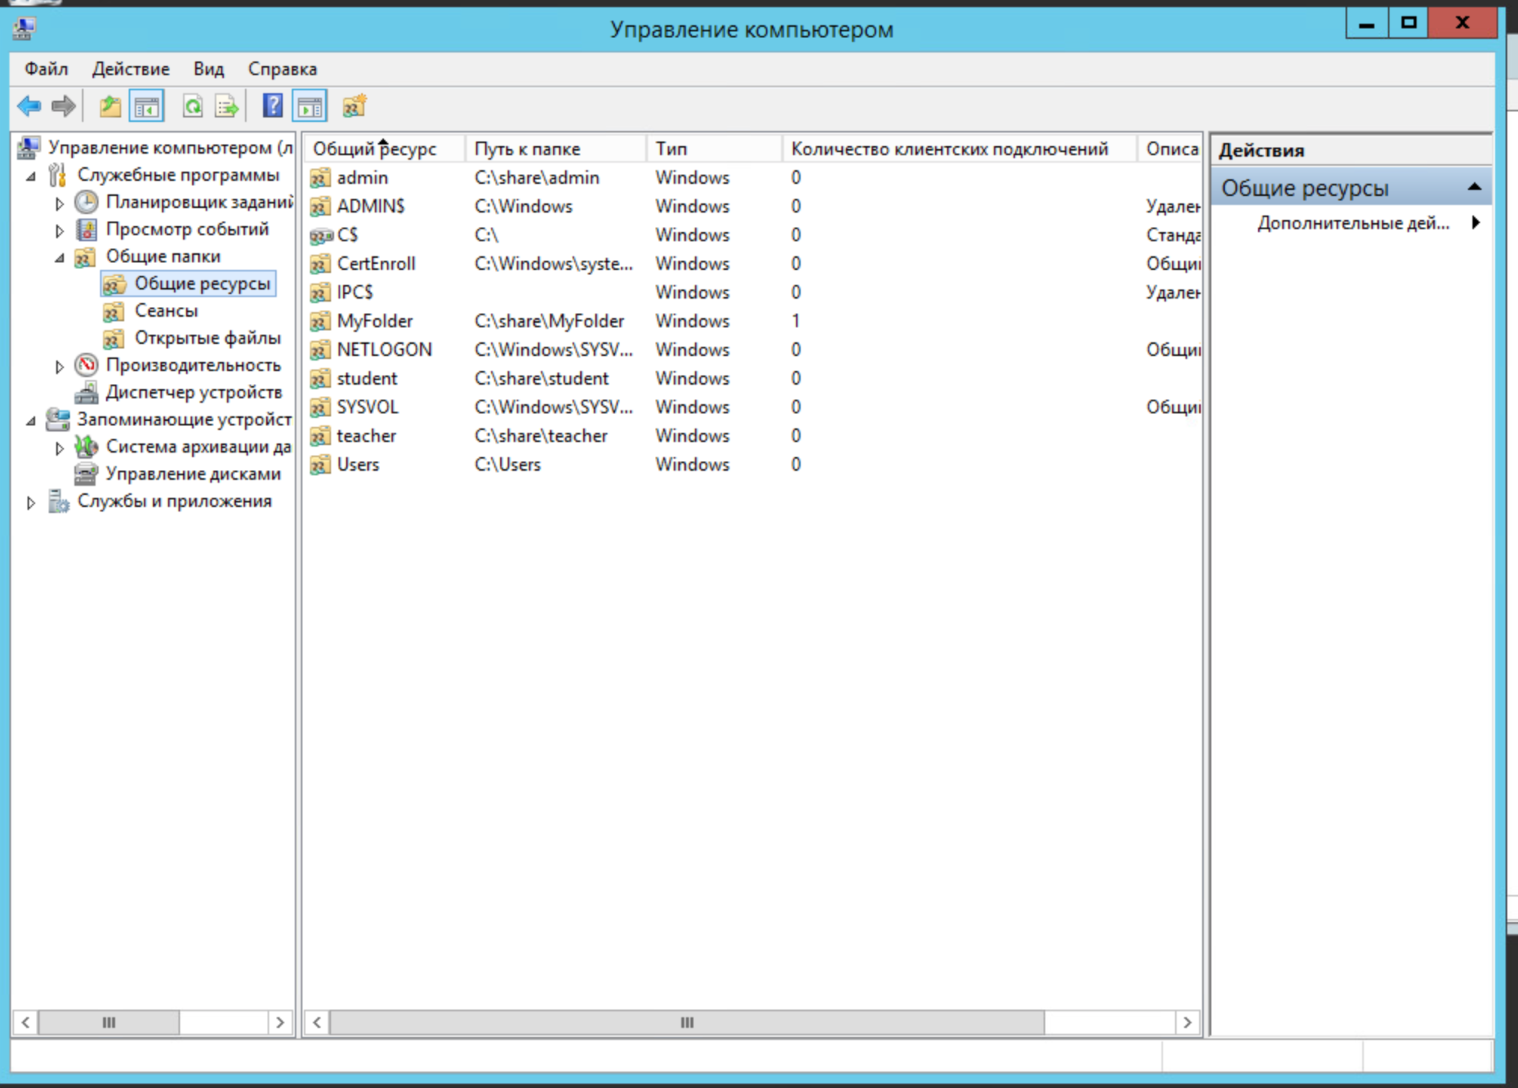
\includegraphics[scale=0.6]{6.png}
    \end{center}

    \newpage
    \textbf{пункт 7}
    \begin{center}
        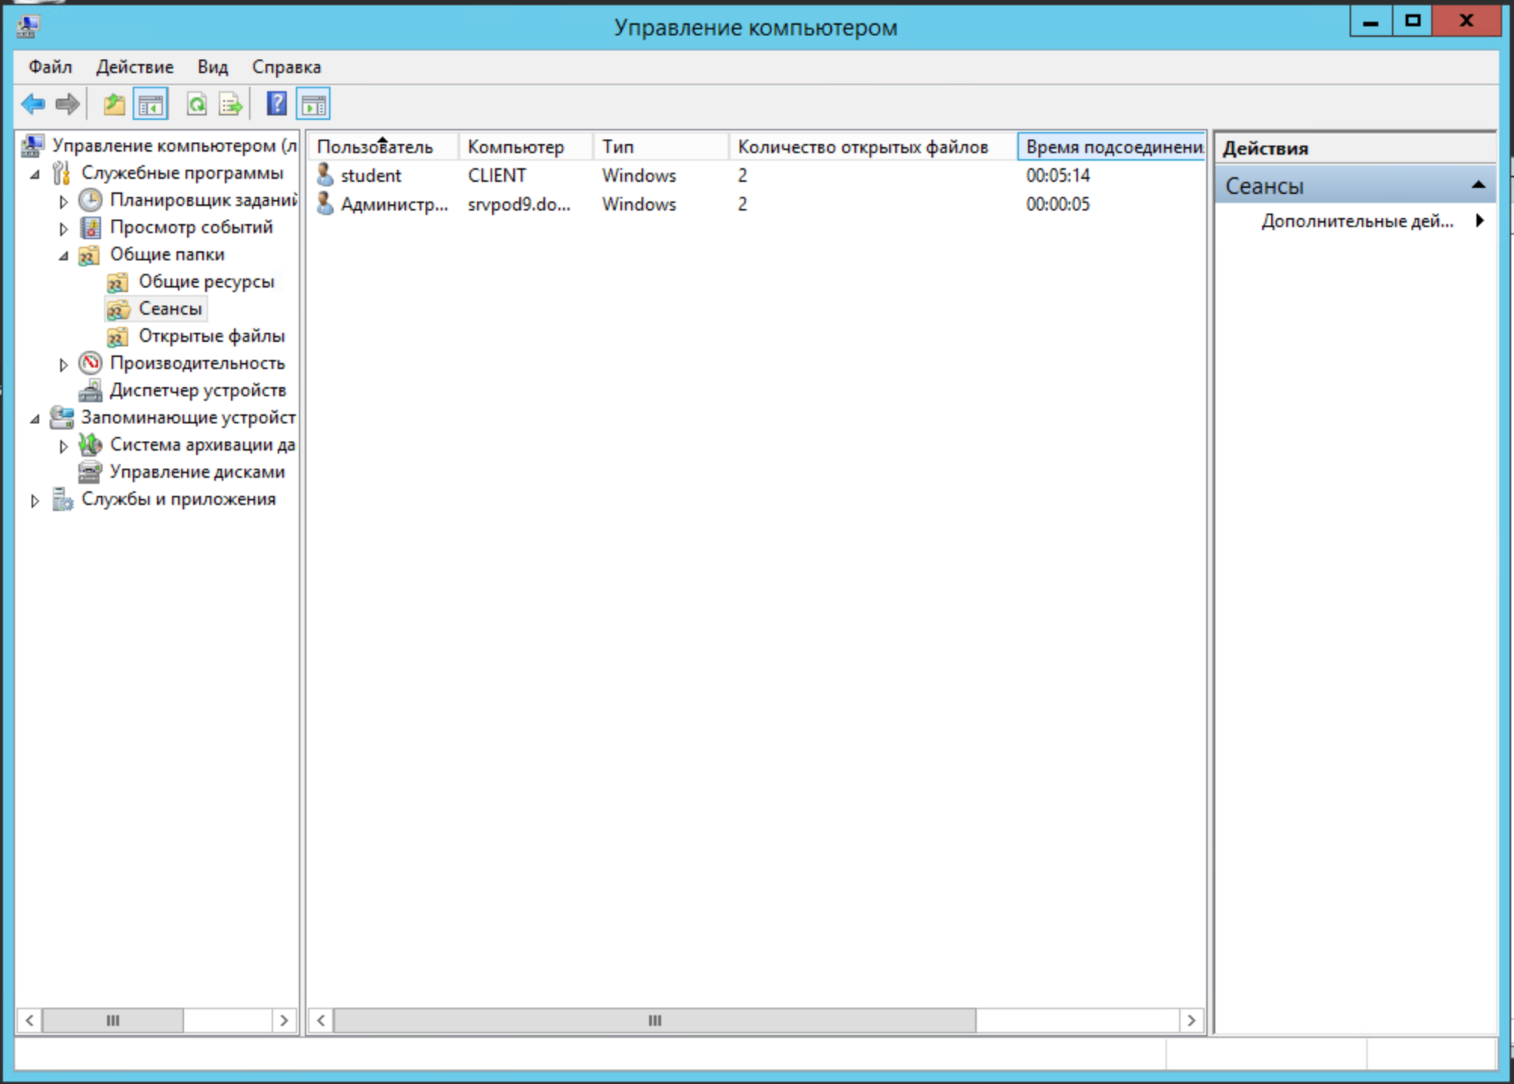
\includegraphics[scale=0.6]{7.png}
    \end{center}

    \textbf{пункт 8}
    \begin{center}
        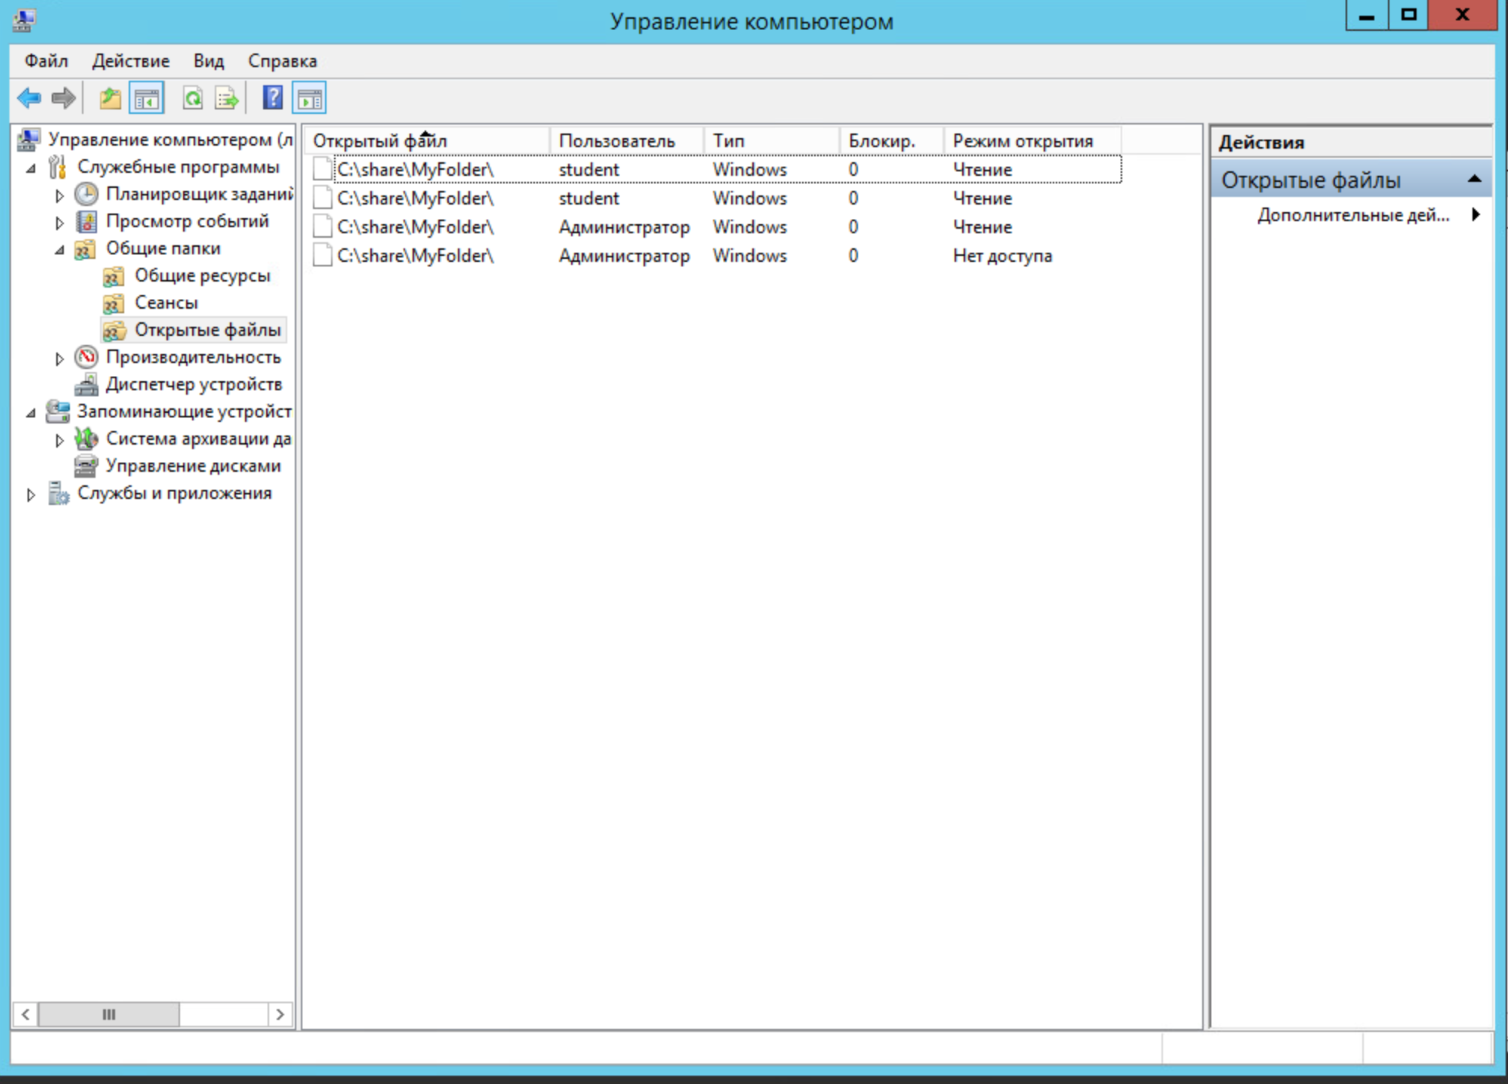
\includegraphics[scale=0.6]{8.png}
    \end{center}

    \newpage
    \textbf{пункт 9}
    \begin{center}
        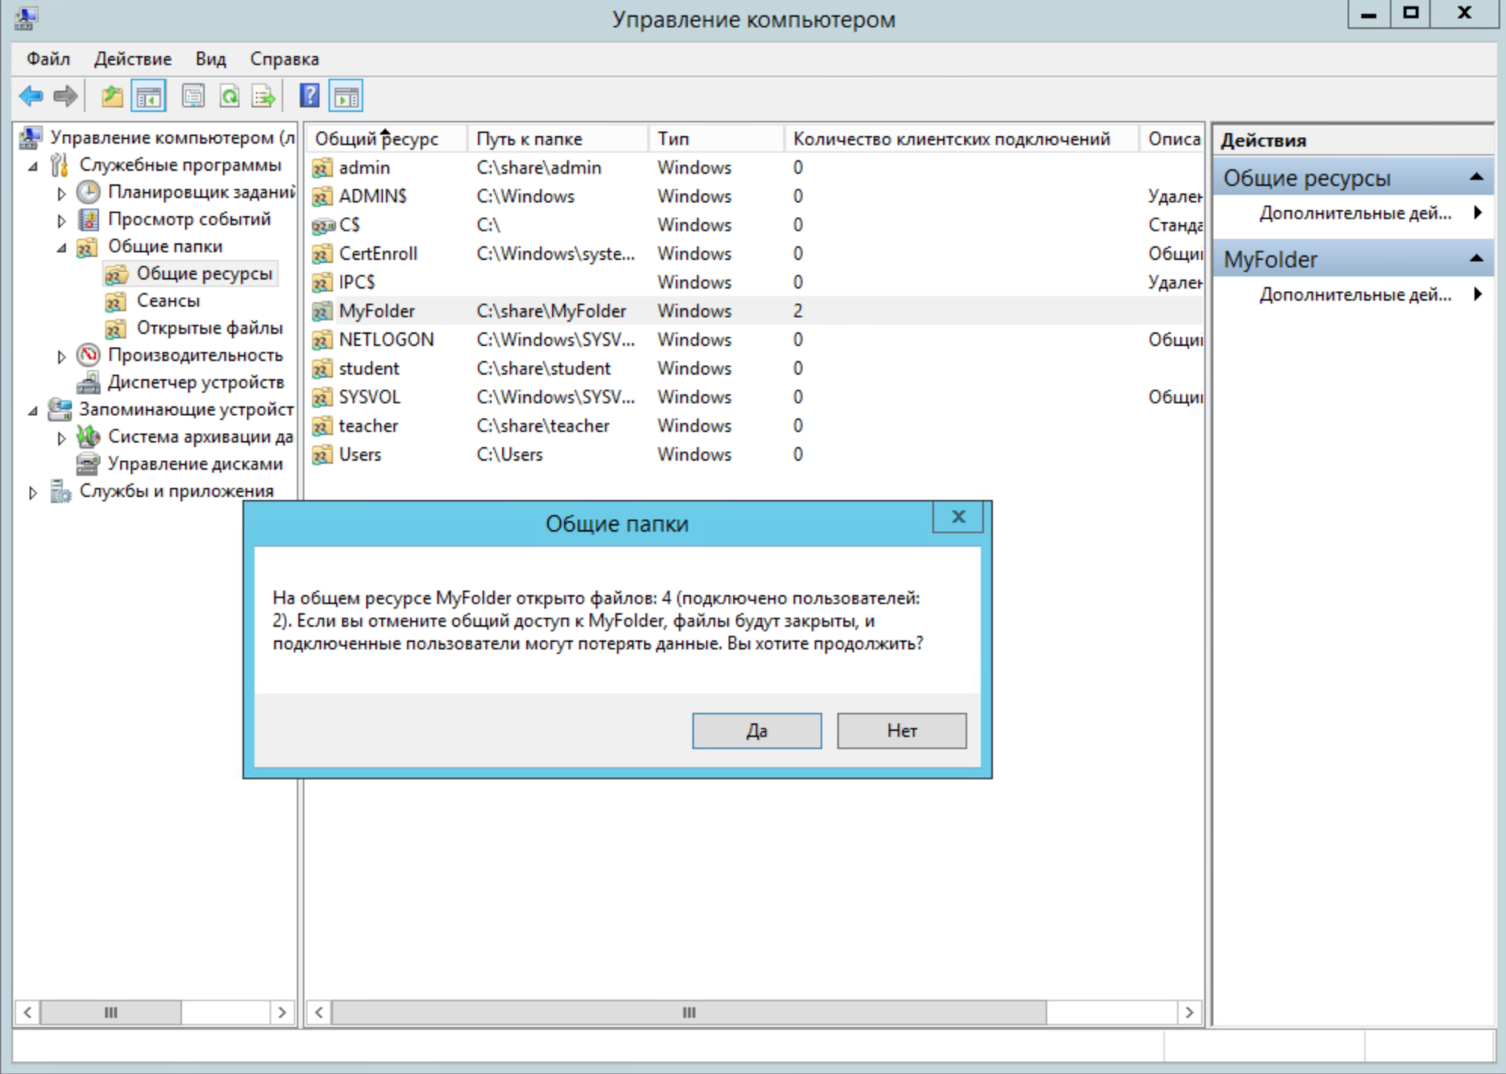
\includegraphics[scale=0.6]{9.png}
    \end{center}

    \textbf{пункт 14}
    \begin{center}
        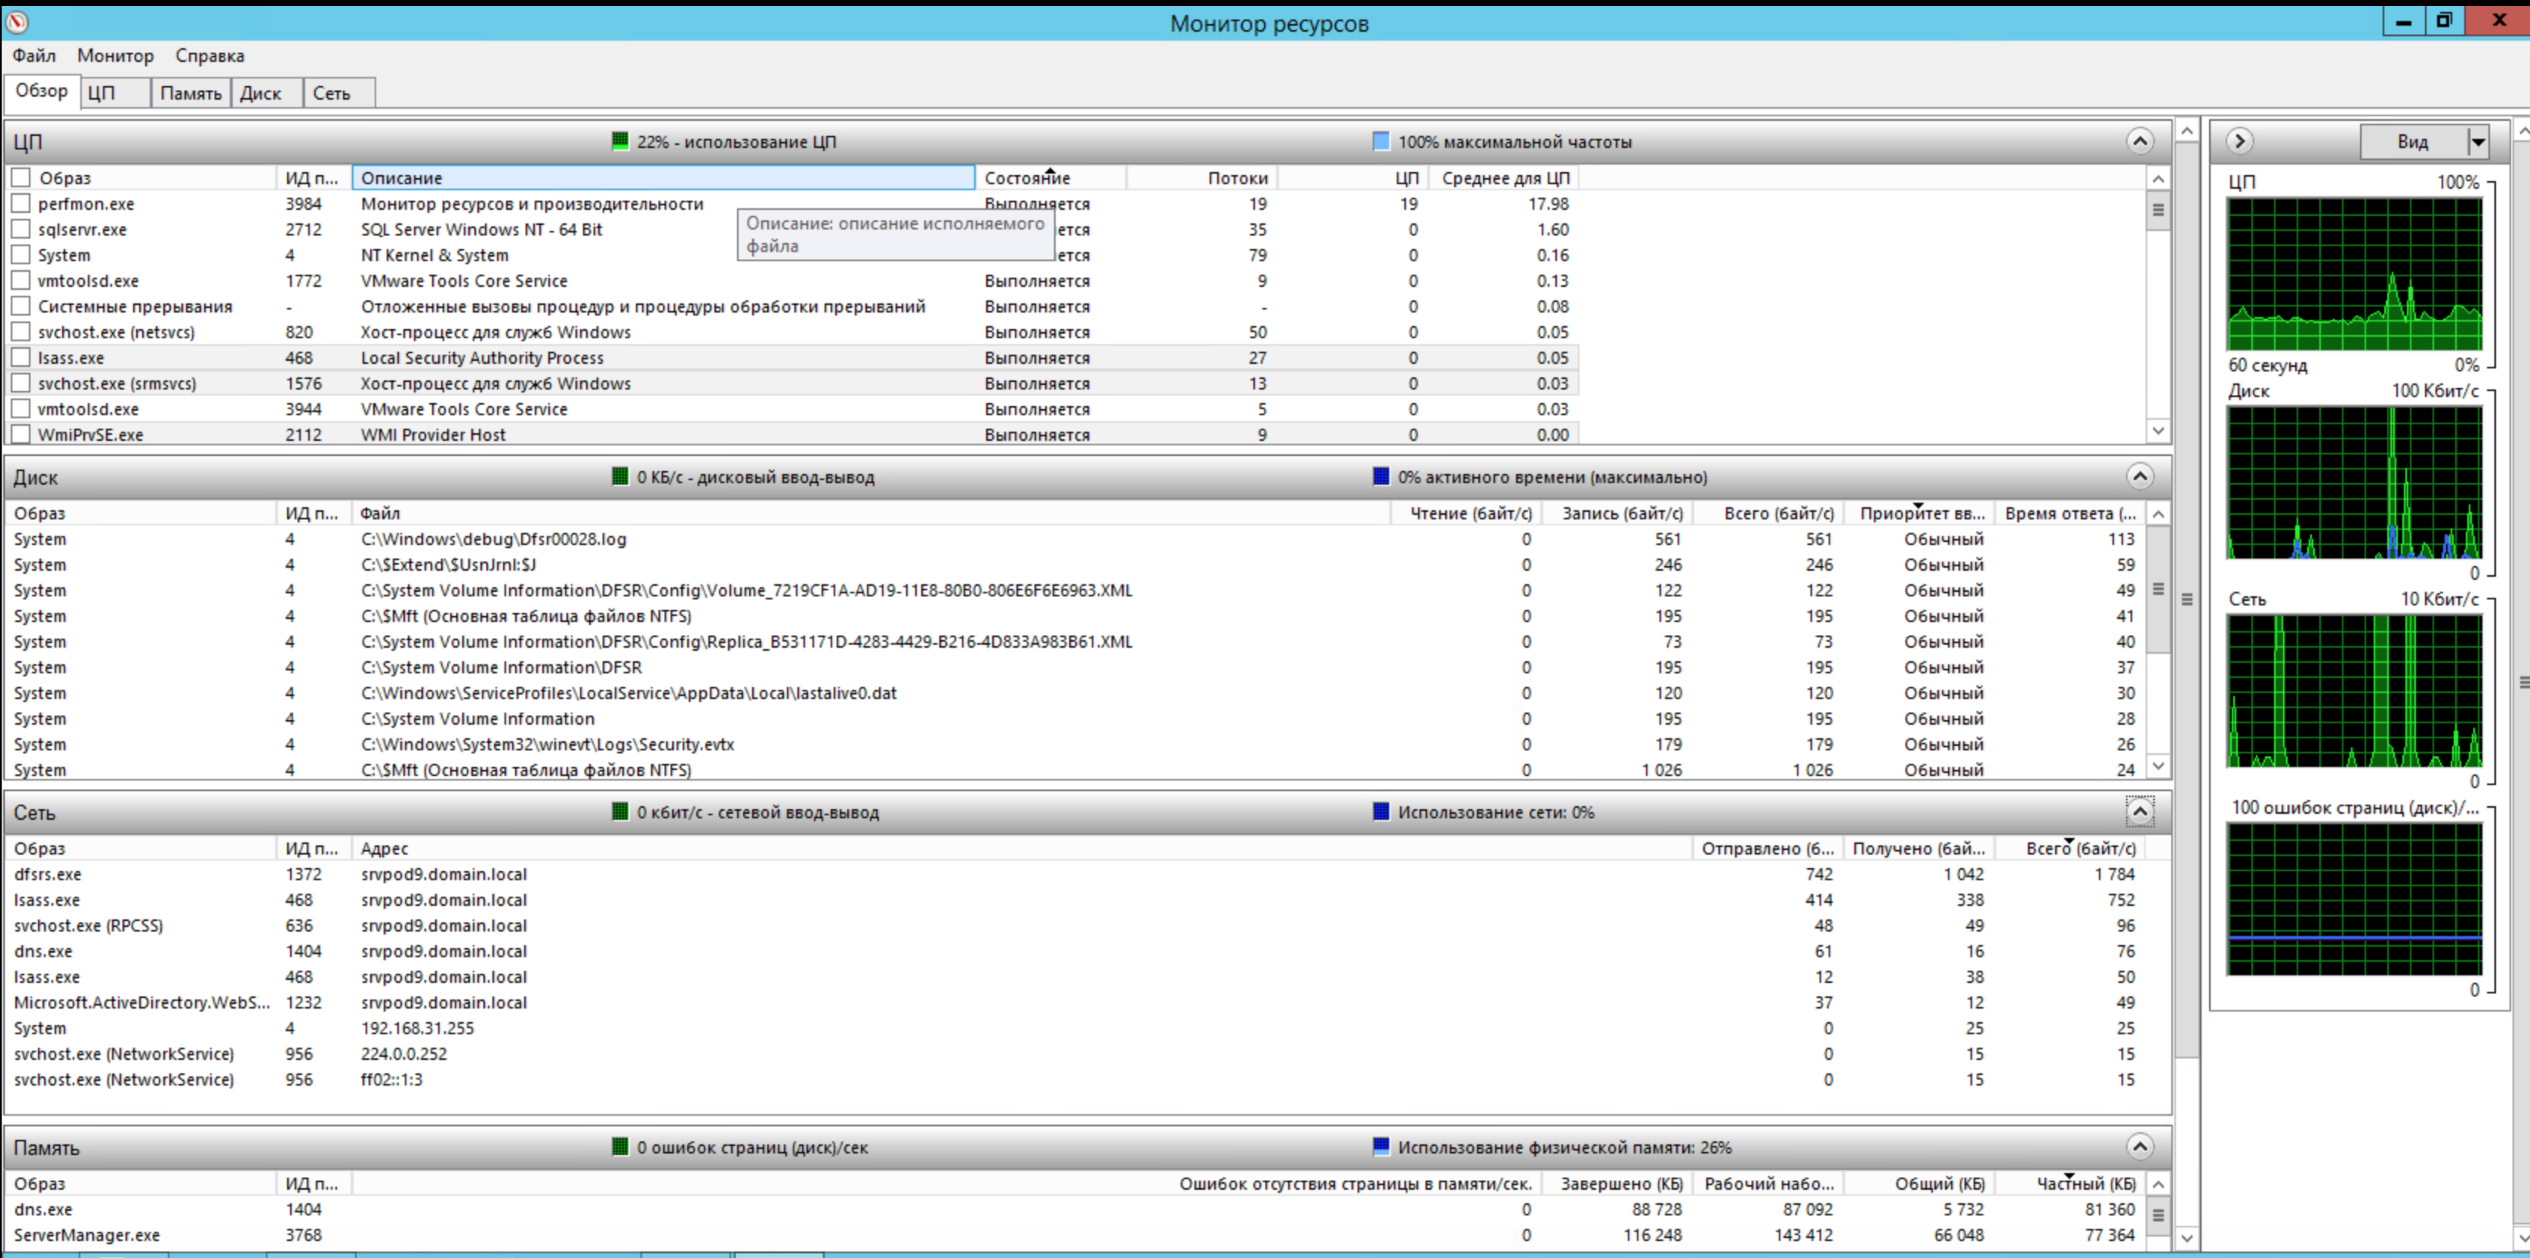
\includegraphics[scale=0.4]{14.png}
    \end{center}
    a. 51\\
    b. ServerManager.exe 143 394 КБ\\
    c. System\\

    \newpage
    \textbf{пункт 19}
    \begin{center}
        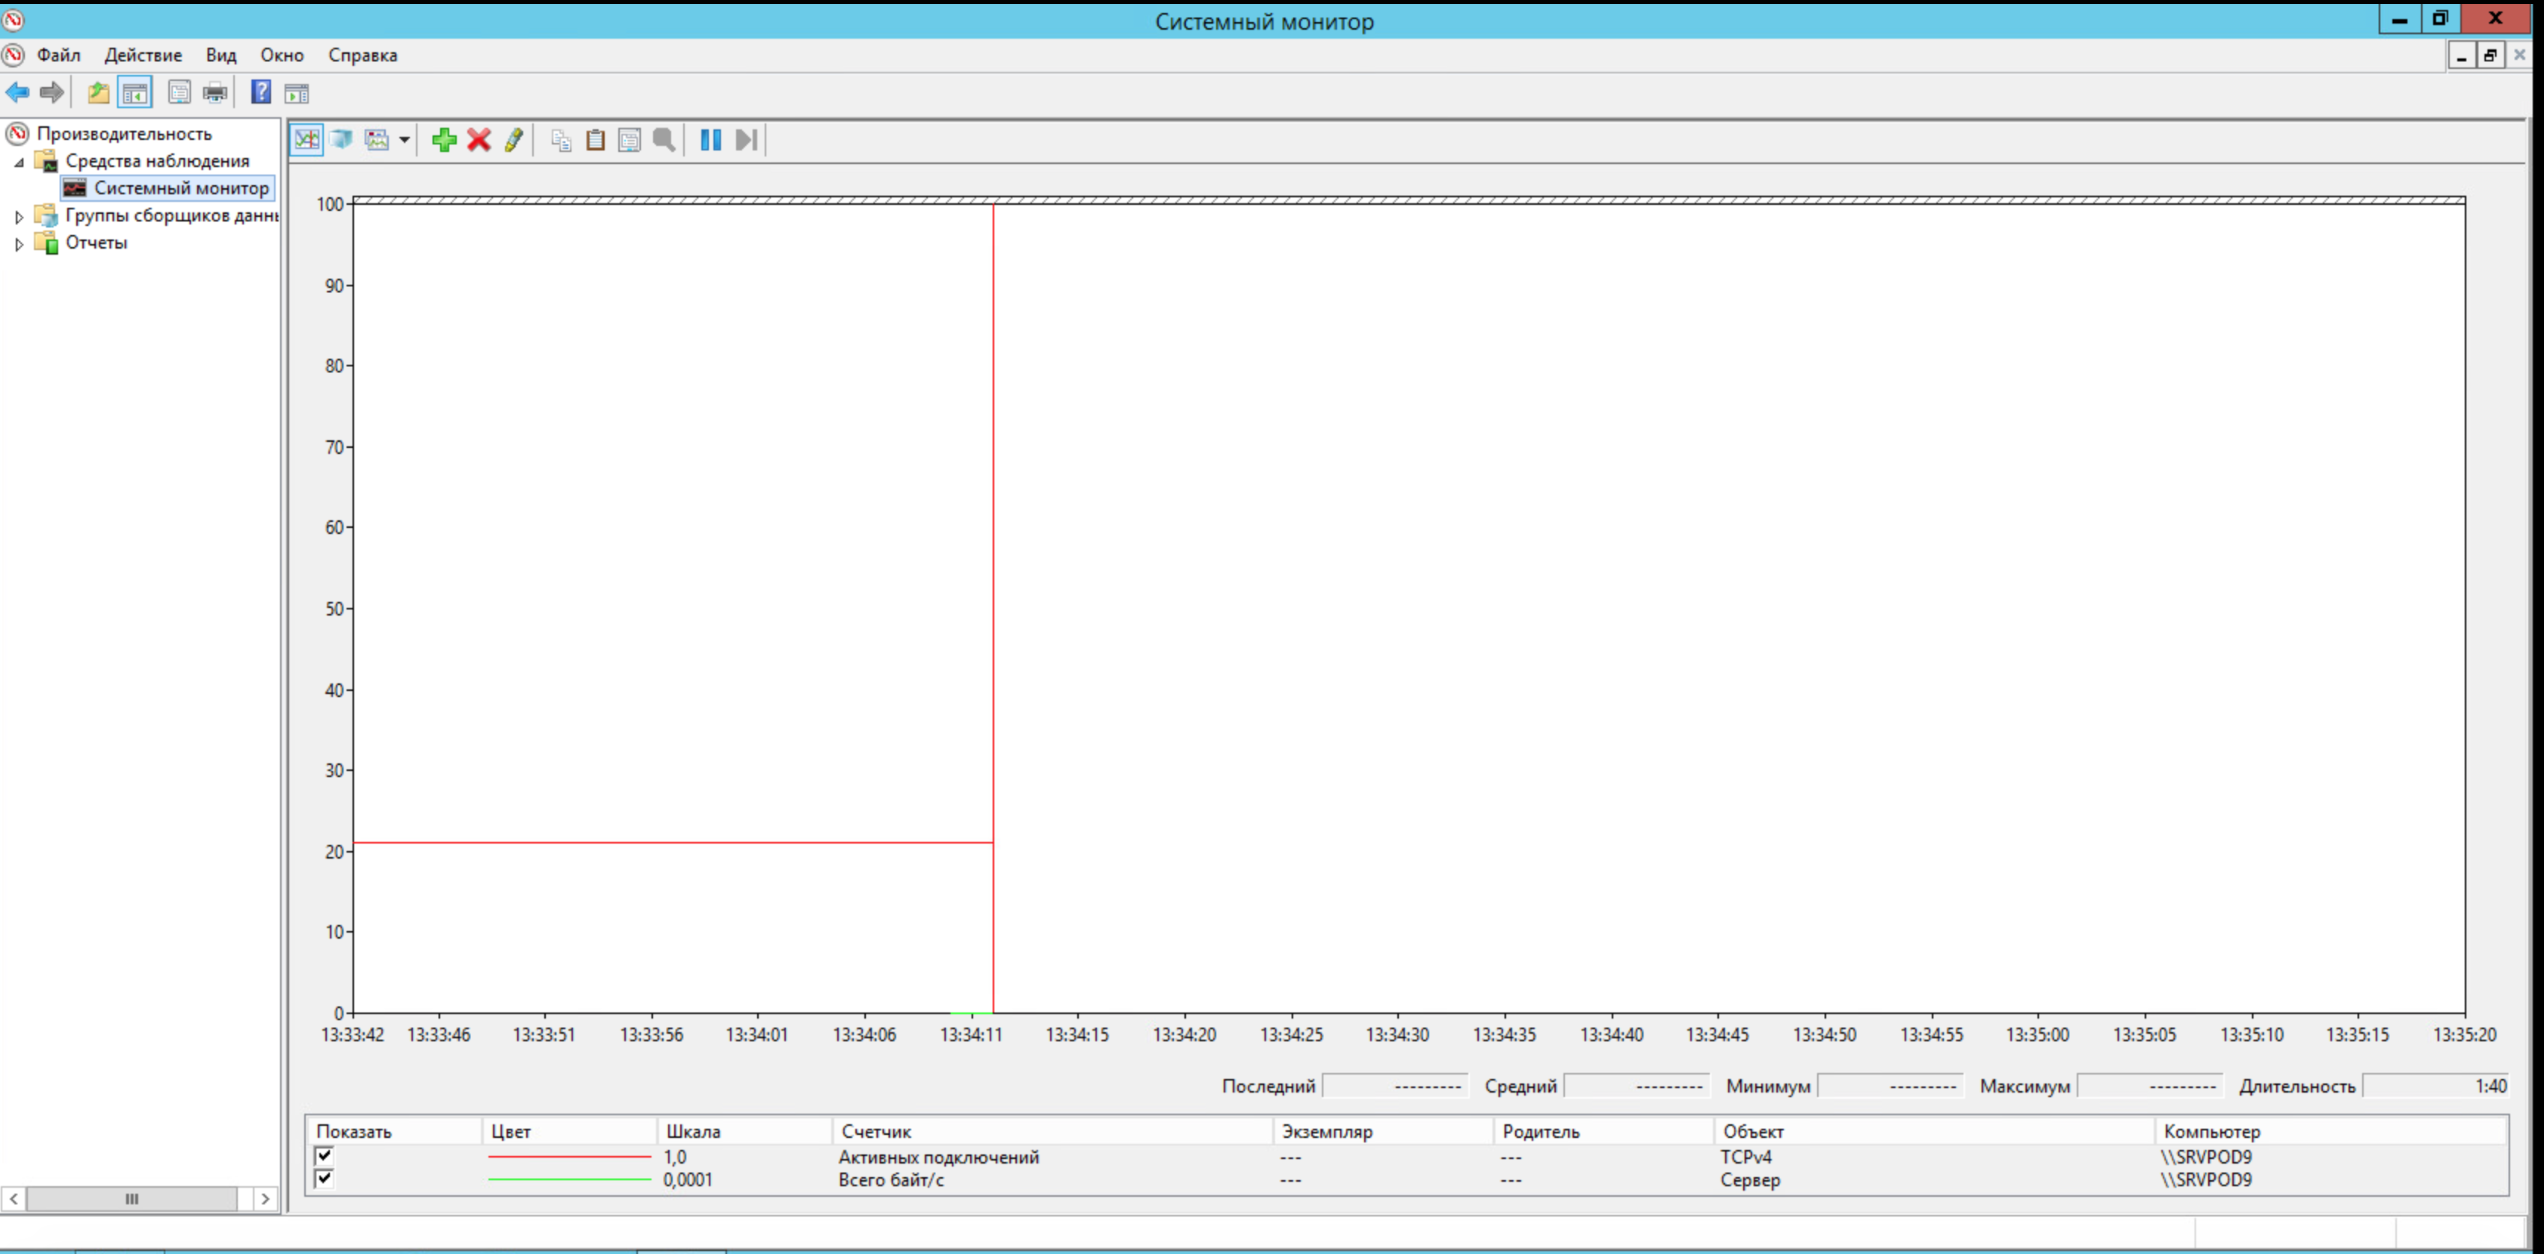
\includegraphics[scale=0.4]{19.png}
    \end{center}

    \textbf{пункт 21}
    \begin{center}
        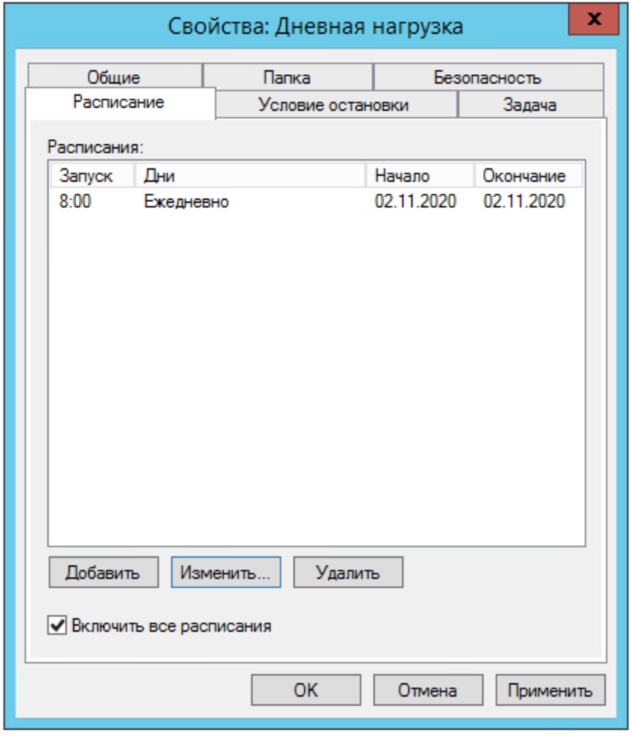
\includegraphics[scale=0.7]{21.1.png}
    \end{center}

    \begin{center}
        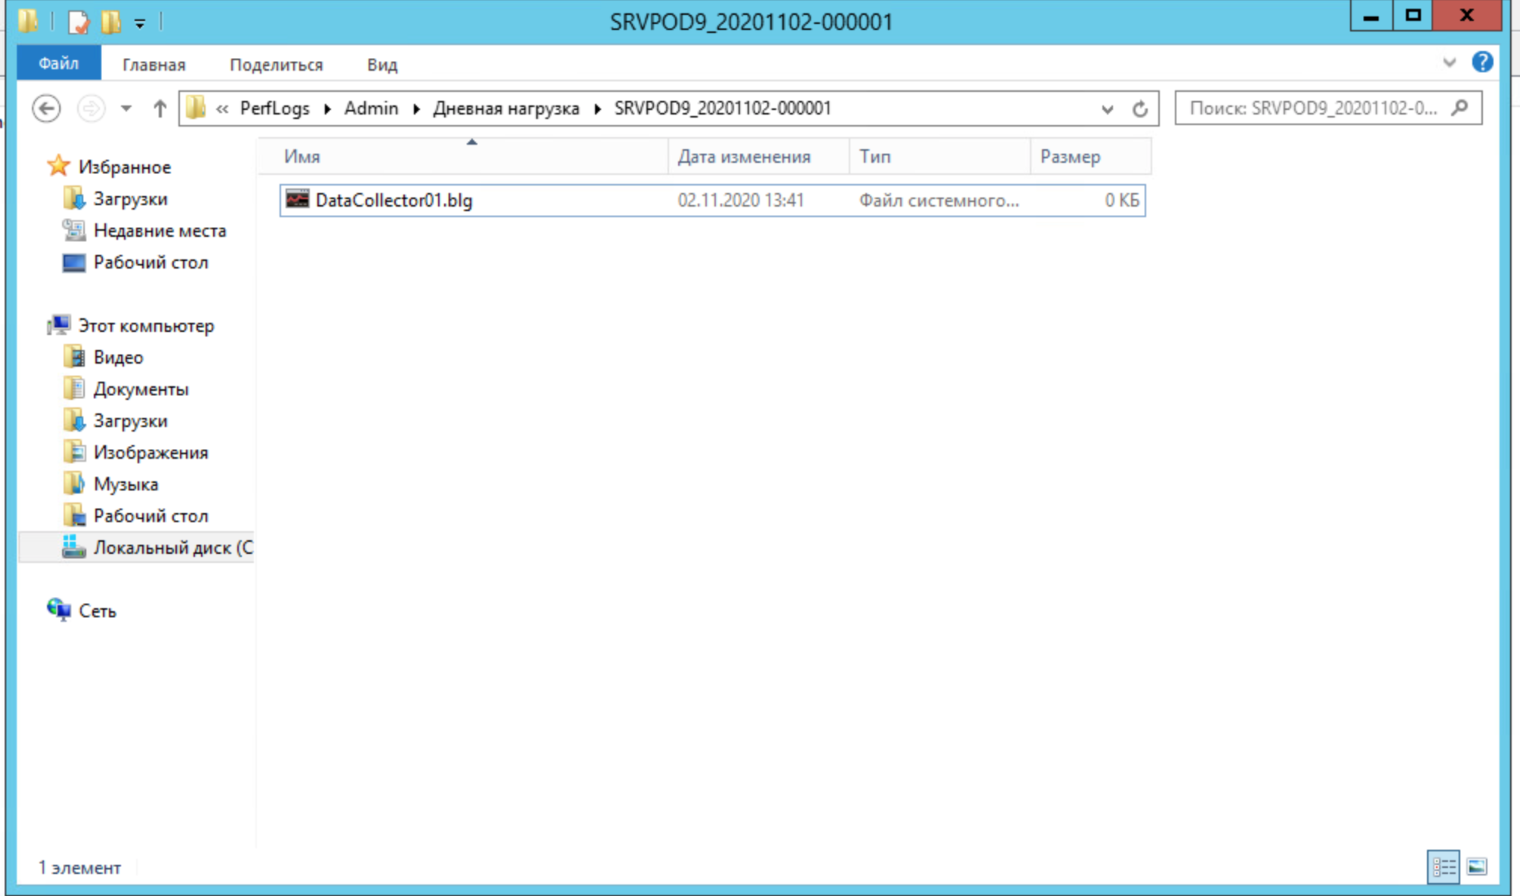
\includegraphics[scale=0.6]{21.2.png}
    \end{center}

    \textbf{пункт 22}
    \begin{center}
        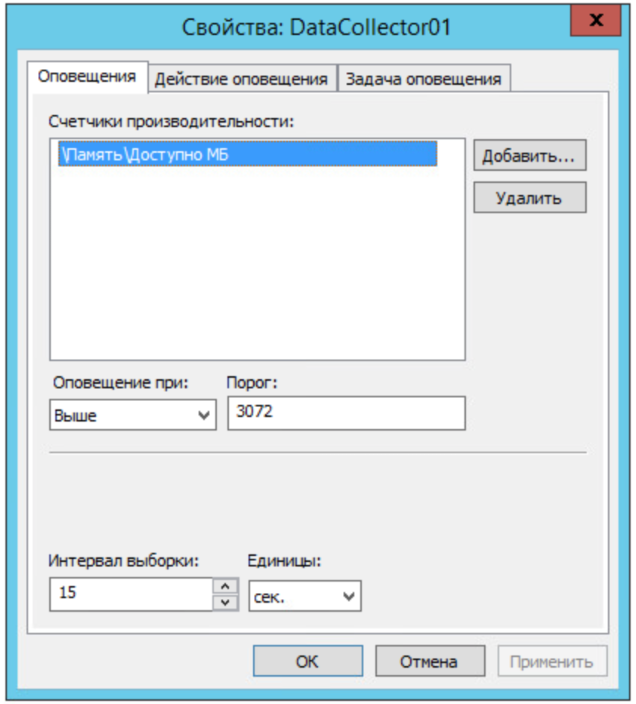
\includegraphics[scale=0.7]{22.png}
    \end{center}

    \newpage
    \textbf{пункт 24}
    \begin{center}
        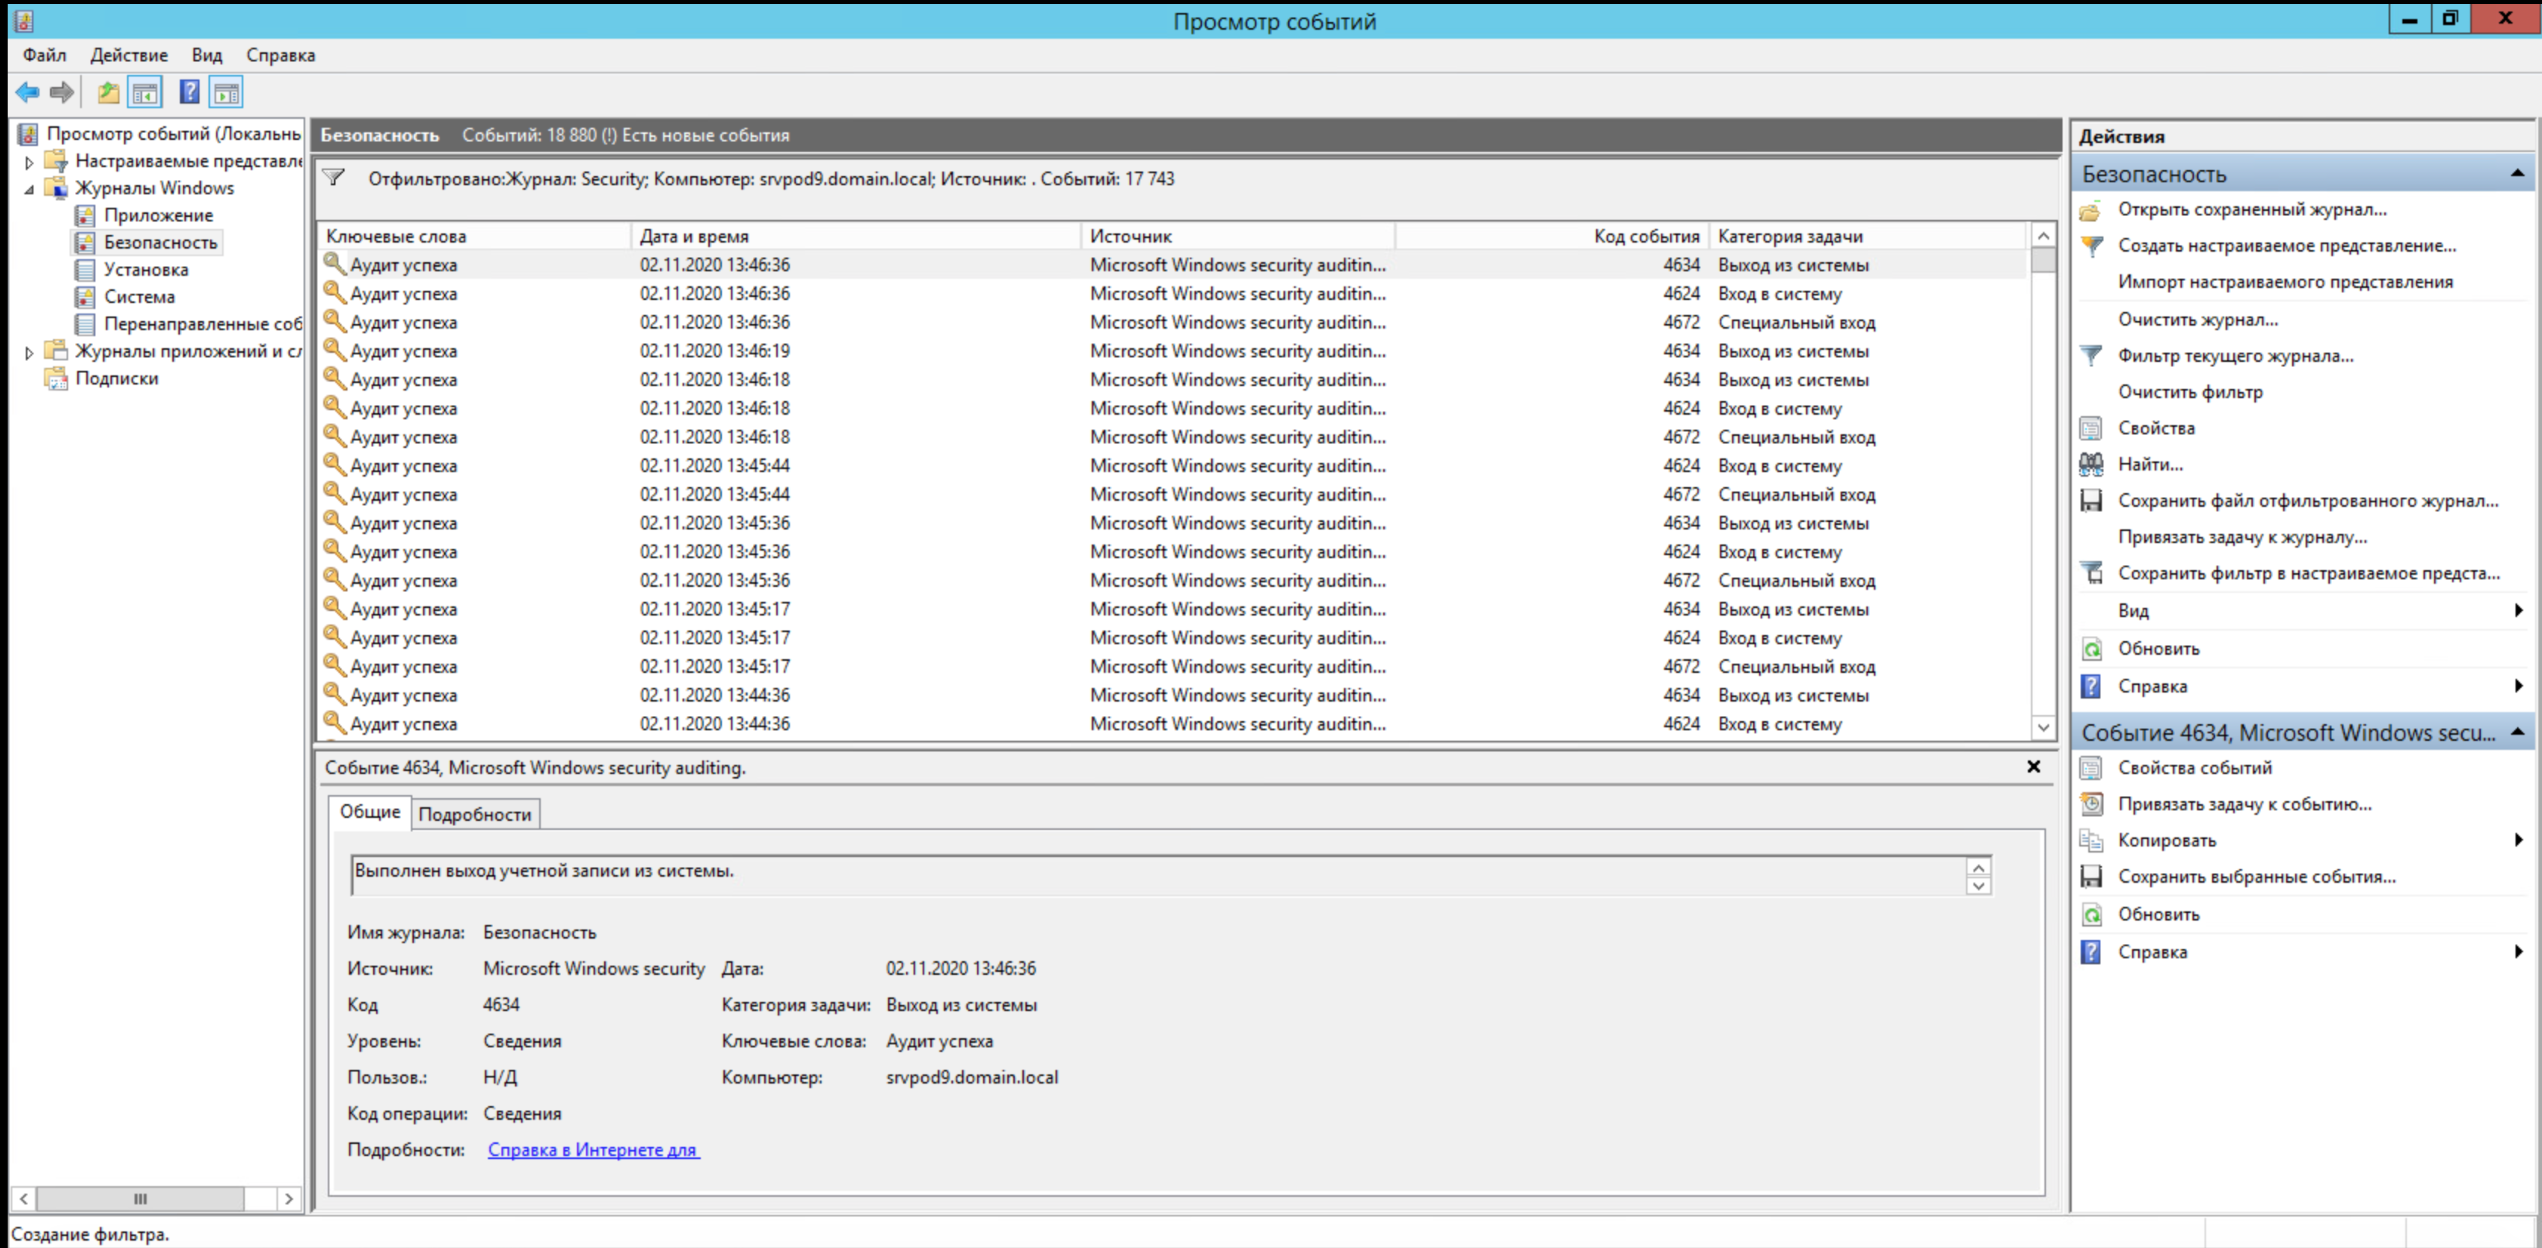
\includegraphics[scale=0.4]{24.b.png}
    \end{center}

    \begin{center}
        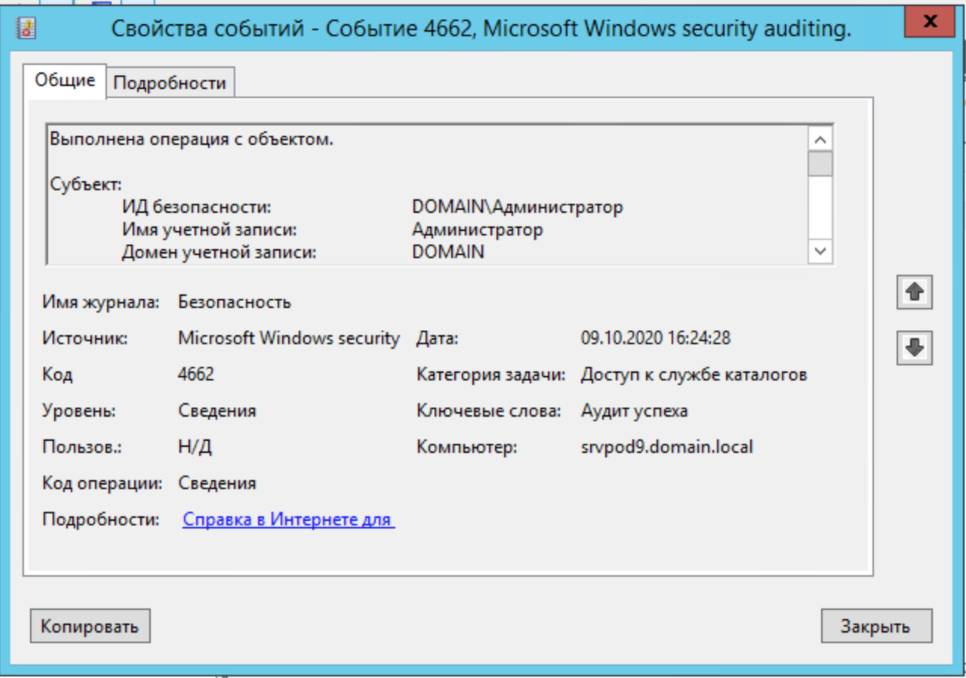
\includegraphics[scale=0.7]{24.c.png}
    \end{center}

    \begin{center}
        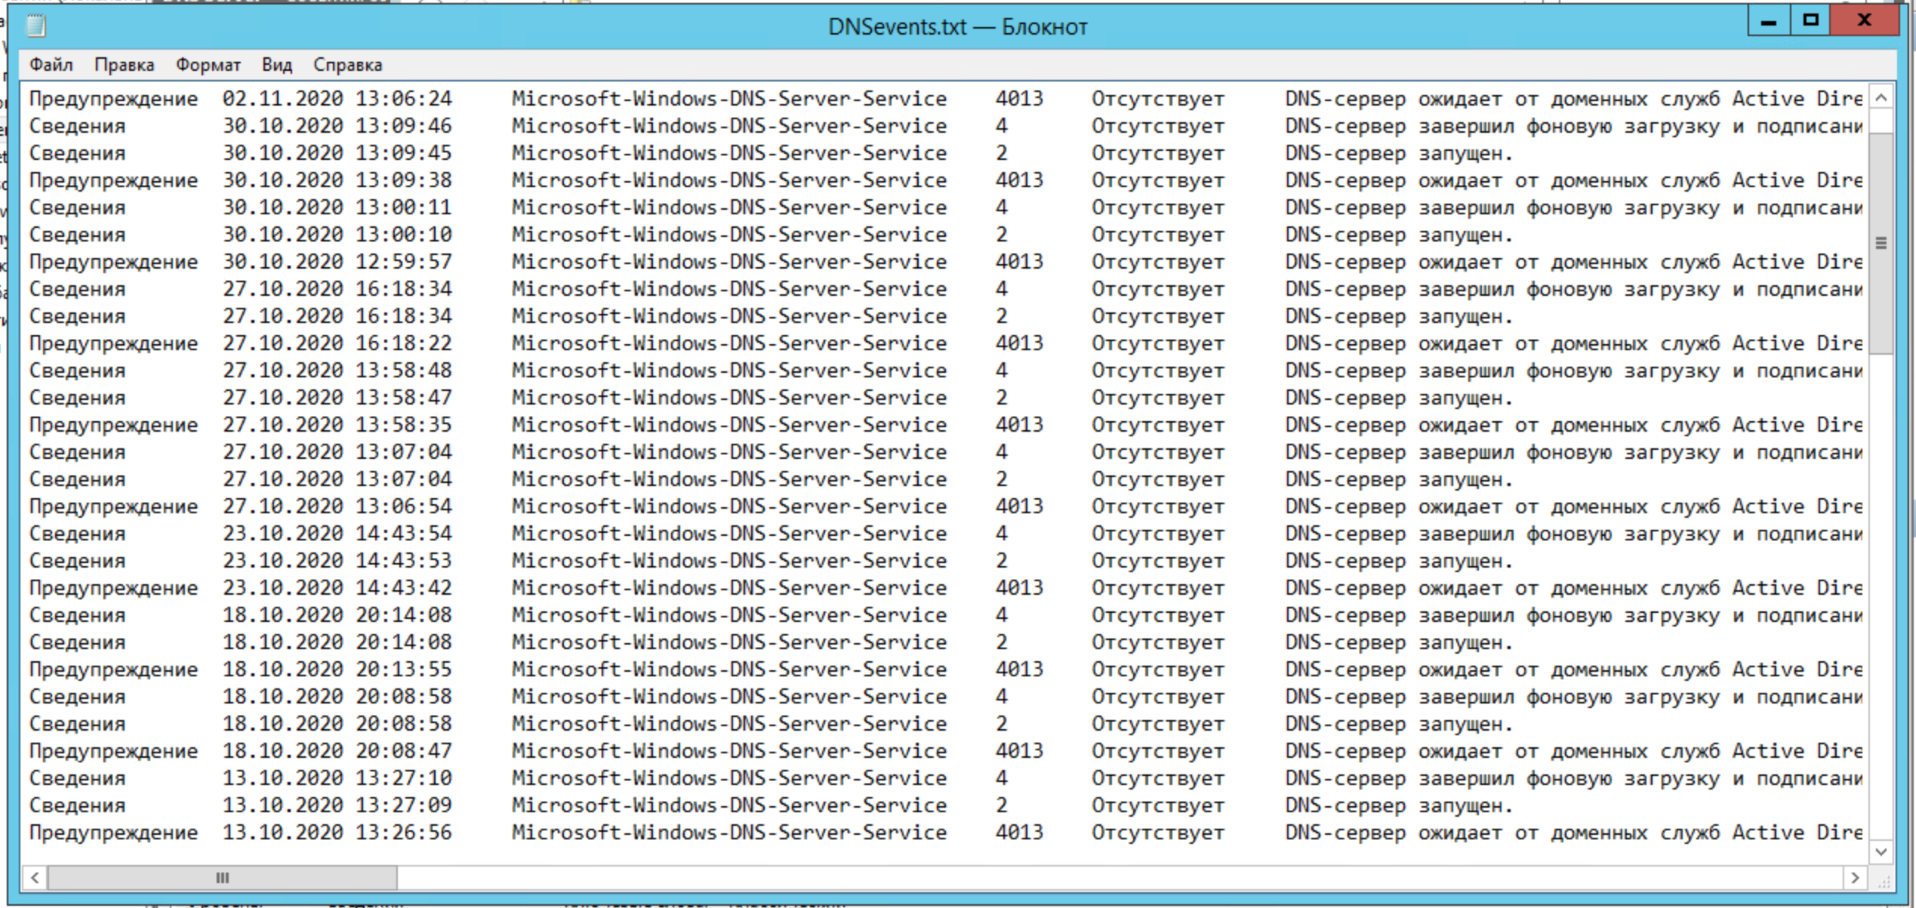
\includegraphics[scale=0.5]{24.d.png}
    \end{center}

    \textbf{Вывод:}

    В ходе данной лабораторной работы мы ознакомились с диспетчером задач и 
    просмотром событий. Также мы научились просматривать различные данные о 
    системе и выполнять их автоматический сбор. Настроили оповещения об 
    изменении параметров компьютера.


\end{document}